% This example uses the 'minted' package, so you need to run the compiler with 
% the '-shell-escape' option, i.e.
% 	pdflatex -shell-escape example.tex
% Additionally, you must have the 'pygmentize' program installed, which is part of 
% the 'Pygments' package (https://pygments.org/)

\documentclass[aspectratio=1610, polish]{beamer}

% Jeśli chcesz otrzymać prezentację w języku polskim, to, powyżej, zamień „english” na „polish”
\usepackage{animate}
\usepackage{mdframed}
\usepackage{graphicx}
\usepackage{babel}
\makeatletter
\usepackage{polski}
\makeatother
\usepackage[utf8]{inputenc}
\usepackage{tikz}
\usetikzlibrary{shapes,arrows,fit,positioning} % Rozszerzenia TikZ
\usepackage{xcolor} % Kolory, w tym niestandardowe jak Dandelion
\usepackage{multicol} % Obsługa wielu kolumn
\usepackage{listings} % We want to put listings
\usepackage{minted}   % We want to put listings
\mode<beamer>{ 	% In the 'beamer' mode
	\definecolor{links}{HTML}{2A1B81}
	\hypersetup{
		pdfpagemode=FullScreen,                 % Enable Full screen mode
		colorlinks,
		linkcolor=,
		urlcolor=links
	}
	\usetheme[parttitle=rightfooter]{AGH}       % Show part title in right footer
	% \usetheme[nosidebar]{AGH}                  % Do not show sidebar on non-title slides
	%\usetheme[nosidebar, margins=1em]{AGH}     % Do not show sidebar on non-title slides and set both margins (left / right) to 1em
	% \usetheme[dark]{AGH}                       % Use dark background
	% \usetheme[dark, parttitle=leftfooter]{AGH} % Use dark background and show part title in left footer
}
\mode<handout>{	% In the 'handout' mode
	\hypersetup{pdfpagemode=None}		
	\usepackage{pgfpages}
	\pgfpagesuselayout{4 on 1}[a4paper,border shrink=5mm,landscape]	% Show 4 slides on 1 page
	\pgfpageslogicalpageoptions{1}{border code=\pgfusepath{stroke}}
	\pgfpageslogicalpageoptions{2}{border code=\pgfusepath{stroke}}
	\pgfpageslogicalpageoptions{3}{border code=\pgfusepath{stroke}}
	\pgfpageslogicalpageoptions{4}{border code=\pgfusepath{stroke}}
  	\usetheme{boxes}
  	\addheadbox{structure}{\quad\insertpart\hfill\insertsection\hfill\insertsubsection\qquad}          % Content of header
 	\addfootbox{structure}{\quad\insertshortauthor\hfill\insertframenumber\hfill\insertsubtitle\qquad} % Content of footer
}

\AtBeginPart{ % At begin part: display its name
	\frame{\partpage}
} 
\author[Maciej Kmąk \& Michał Szymocha]{Maciej Kmąk \and Michał Szymocha}
\date{}
\title{Struktury QuadTree i Kd-drzewa}
\institute[AGH]{
        Wydział Informatyki AGH
}
%%%%%%%%%%% Configuration of the listings package %%%%%%%%%%%%%%%%%%%%%%%%%%
% Source: https://en.wikibooks.org/wiki/LaTeX/Source_Code_Listings#Using_the_listings_package
%%%%%%%%%%%%%%%%%%%%%%%%%%%%%%%%%%%%%%%%%%%%%%%%%%%%%%%%%%%%%%%%%%%%%%%%%%%%
\lstset{ %
  backgroundcolor=\color{white},   % choose the background color
  basicstyle=\footnotesize,        % the size of the fonts that are used for the code
  breakatwhitespace=false,         % sets if automatic breaks should only happen at whitespace
  breaklines=true,                 % sets automatic line breaking
  captionpos=b,                    % sets the caption-position to bottom
  commentstyle=\color{green},      % comment style
  deletekeywords={...},            % if you want to delete keywords from the given language
  escapeinside={\%*}{*)},          % if you want to add LaTeX within your code
  extendedchars=true,              % lets you use non-ASCII characters; for 8-bits encodings only, does not work with UTF-8
  frame=single,	                   % adds a frame around the code
  keepspaces=true,                 % keeps spaces in text, useful for keeping indentation of code (possibly needs columns=flexible)
  keywordstyle=\color{blue},       % keyword style
  morekeywords={*,...},            % if you want to add more keywords to the set
  numbers=left,                    % where to put the line-numbers; possible values are (none, left, right)
  numbersep=5pt,                   % how far the line-numbers are from the code
  numberstyle=\tiny\color{gray},   % the style that is used for the line-numbers
  rulecolor=\color{black},         % if not set, the frame-color may be changed on line-breaks within not-black text (e.g. comments (green here))
  showspaces=false,                % show spaces everywhere adding particular underscores; it overrides 'showstringspaces'
  showstringspaces=false,          % underline spaces within strings only
  showtabs=false,                  % show tabs within strings adding particular underscores
  stepnumber=2,                    % the step between two line-numbers. If it's 1, each line will be numbered
  stringstyle=\color{cyan},        % string literal style
  tabsize=2,	                   % sets default tabsize to 2 spaces
  title=\lstname,                  % show the filename of files included with \lstinputlisting; also try caption instead of title
                                   % needed if you want to use UTF-8 Polish chars
  literate={ą}{{\k{a}}}1
           {Ą}{{\k{A}}}1
           {ę}{{\k{e}}}1
           {Ę}{{\k{E}}}1
           {ó}{{\'o}}1
           {Ó}{{\'O}}1
           {ś}{{\'s}}1
           {Ś}{{\'S}}1
           {ł}{{\l{}}}1
           {Ł}{{\L{}}}1
           {ż}{{\.z}}1
           {Ż}{{\.Z}}1
           {ź}{{\'z}}1
           {Ź}{{\'Z}}1
           {ć}{{\'c}}1
           {Ć}{{\'C}}1
           {ń}{{\'n}}1
           {Ń}{{\'N}}1
}

\begin{document}

\begin{frame}[t]
    \maketitle
\end{frame}

\begin{frame}{Plan prezentacji}
    \tableofcontents
\end{frame}

\begin{section}{Przedstawienie problemu}
    
\begin{frame}
    \frametitle{Problem wyszukiwania punktów w obszarze}
    \textbf{Opis problemu:}
    \begin{itemize}
        \item Dane są punkty $P_1 = (x_1, y_1)$ oraz $P_2 = (x_2, y_2)$, które definiują prostokąt w przestrzeni dwuwymiarowej.
        \item Zbiór $P$ to punkty w przestrzeni dwuwymiarowej.
        \item Zadanie polega na znalezieniu wszystkich punktów $Q \subseteq P$, dla których:
        \[
        x_1 < x_Q < x_2 \quad \text{oraz} \quad y_1 < y_Q < y_2.
        \]
    \end{itemize}
    \pause
    \vspace{0.5cm}
    
    \textbf{Cel projektu:}
    \begin{itemize}
        \item Zaimplementowanie struktur danych \texttt{QuadTree} i \texttt{KdTree}.\\
            \biitem Struktury mają umożliwiać szybkie odpowiadanie na zapytania o punkty znajdujące się w zadanym prostokątnym obszarze.
        \item Porównanie wydajności zaimplementowanych struktur.
    \end{itemize}
\end{frame}

\begin{frame}{Propozycje rozwiązania}
Możemy odpowiedzieć na to pytanie, przechodząc po całym zbiorze punktów, sprawdzając warunek dla każdego z nich lub skorzystać z bardziej zaawansowanych struktur, takich jak: \texttt{QuadTree} i \texttt{Kd-Drzewa}
\pause
\vspace{0.5cm}
\\
\textbf{\large Porównanie algorytmów:}

\begin{itemize}
    \item \textbf{Algorytm podstawowy -- rozwiązanie naiwne:}
    \begin{itemize}
        \item Złożoność czasowa: \( O(n) \)
    \end{itemize}
    \item \textbf\texttt{QuadTree:}
    \begin{itemize}
        \item Złożoność czasowa: \( O(\log n + k) \)
    \end{itemize}
    \item \textbf\texttt{Kd-Drzewa:}
    \begin{itemize}
        \item Złożoność czasowa: \( O(\sqrt{n} + k) \)
    \end{itemize}
\end{itemize}

\vspace{0.5cm}
\textit{\footnotesize $n$ -- liczba punktów zbioru $P$} \\
\textit{\footnotesize $k$ -- liczba punktów wynikowych}
\end{frame}

\begin{frame}[fragile]{Rozwiązanie naiwne}
        Sprawdzamy każdy punkt, takie podejście ma złożoność czasową $O(n)$. \\
    
        \pause
        Dla prostokąta $R = [x_1, x_2] \times [y_1, y_2]$:
        \begin{minted}{python}
    filter(lambda p: x_1 <= p[0] <= x_2 and y_1 <= p[1] <= y_2, P)
        \end{minted}
\end{frame}
\end{section}
\begin{section}{Drzewa czwórkowe \textt{QuadTree}}
    \begin{frame}{Struktura danych \texttt{QuadTree}}
        
        \texttt{QuadTree} to struktura danych umożliwiająca przechowywanie punktów w przestrzeni dwuwymiarowej.  
        Jej głównym zadaniem jest rekurencyjny podział przestrzeni na mniejsze części poprzez dzielenie jej na cztery równe ćwiartki. 
        \vspace{0.5cm}
        \pause
        \begin{itemize}
            \item Każda z tych ćwiartek może być dalej dzielona na kolejne cztery części, dopóki liczba punktów w danym obszarze nie przekroczy zdefiniowanej maksymalnej pojemności węzła \textt{max\_capacity}.
            \pause
            \item Węzły drzewa reprezentują prostokątne obszary przestrzeni.
            \pause
            \item Liście to najmniejsze prostokąty, które nie są już dzielone z powodu ograniczenia liczby punktów.
        \end{itemize}

    \end{frame}


    \begin{frame}
        \frametitle{\texttt{QuadTree} -- teoretyczna złożoność}
            
        \begin{itemize}
            \item \textbf{Budowa struktury:}  
            \(O(n \log n)\), gdzie \(n\) to liczba punktów w zbiorze, przy założeniu równomiernego rozkładu punktów.
        \pause
        \vspace{0.5cm}
            \item \textbf{Wyszukiwanie punktów w zadanym obszarze:}  
        \(O(\log n + k)\), gdzie:
        \begin{itemize}
            \item \(\log n\) to maksymalna głębokość drzewa w dobrze zrównoważonej strukturze,
            \item \(k\) to liczba punktów wewnątrz zadanego obszaru.  
        \end{itemize}
        Dzięki rekurencyjnemu podziałowi przestrzeni wyszukiwanie jest ograniczone tylko do podobszarów przecinających zadany obszar, co znacząco poprawia efektywność.
        \end{itemize}
    
    \end{frame}
\begin{frame}{Budowa \texttt{QuadTree} (opis kroków)}

\begin{mdframed}
\textbf{Krok 1: Obliczenie prostokąta obejmującego punkty}\\[3pt]
Wyznacz prostokąt graniczny, który obejmuje wszystkie punkty wejściowe.
ustaw go jako korzeń drzewa.
\end{mdframed}

\begin{mdframed}
\textbf{Krok 2: Sprawdzenie liczby punktów}\\[3pt]
Jeśli liczba unikalnych punktów w prostokącie jest mniejsza lub równa \\\texttt{maks\_pojemność}, zakończ podział. Węzeł staje się liściem i przechowuje punkty.
\end{mdframed}

\begin{mdframed}
\textbf{Krok 3: Podział prostokąta na ćwiartki}\\[3pt]
Wyznacz środek prostokąta jako płaszczyzny podziału i podziel punkty na cztery podzbiory: Dół-lewo (SW), Dół-prawo (SE), Góra-lewo (NW), Góra-prawo (NE).
\end{mdframed}

\end{frame}
\begin{frame}{Budowa \texttt{QuadTree} (opis kroków) -- cd.}
\begin{mdframed}
\textbf{Krok 4: Rekurencyjny podział}\\[3pt]
Dla każdej ćwiartki utwórz węzeł podrzędny, przypisz do niego punkty należące do tej ćwiartki, i powtarzaj proces, dopóki liczba punktów w węźle przekracza \texttt{maks\_pojemność}.
\end{mdframed}

\begin{mdframed}
\textbf{Krok 5: Zakończenie}\\[3pt]
Węzły zawierające \texttt{maks\_pojemność} punktów lub mniej stają się liśćmi, a drzewo zostaje zbudowane.
\end{mdframed}

\end{frame}

\begin{frame}{\testtt{QuadTree} –- Wizualizacja budowy}

    \centering
    % Adjust the width as needed (e.g., 0.8\linewidth)
    \animategraphics[
        autoplay,    % Start playing automatically
        loop,        % Loop the animation continuously
        controls,
        width=0.71\linewidth
    ]{3}{gif_quad/frame_}{1}{43}
    % Parameters:
    % 10       - Frame rate (frames per second)
    % frame_   - Prefix of the frame image files
    % 0000     - Starting frame number
    % 0020     - Ending frame number (adjust based on your frames)
\end{frame}

\begin{frame}{Wyszukiwanie w \texttt{QuadTree} (opis kroków)}

\begin{mdframed}
\textbf{Krok 1: Sprawdzenie kolizji prostokątów}\\[3pt]
Sprawdź, czy prostokąt zapytania przecina prostokąt bieżącego węzła.
\end{mdframed}

\begin{mdframed}
\textbf{Krok 2: Przeszukiwanie liścia}\\[3pt]
Jeśli węzeł jest liściem, przeszukaj punkty wewnątrz i zwróć te, które należą do prostokąta zapytania.
\end{mdframed}

\begin{mdframed}
\textbf{Krok 3: Rekurencyjne przeszukiwanie dzieci}\\[3pt]
Jeśli węzeł nie jest liściem, przeszukaj wszystkie jego dzieci, które mają wspólne obszary z prostokątem zapytania.
\end{mdframed}

\begin{mdframed}
\textbf{Krok 4: Zwrócenie wyników}\\[3pt]
Zwróć znalezione punkty lub ich liczności w prostokącie zapytania.
\end{mdframed}

\end{frame}

\begin{frame}{\testtt{QuadTree} –- Wizualizacja przeszukiwania}

    \centering
    % Adjust the width as needed (e.g., 0.8\linewidth)
    \animategraphics[
        autoplay,    % Start playing automatically
        loop,        % Loop the animation continuously
        controls,
        width=0.71\linewidth
    ]{3}{gif_quad_zapytanie/frame_}{1}{22}
    % Parameters:
    % 10       - Frame rate (frames per second)
    % frame_   - Prefix of the frame image files
    % 0000     - Starting frame number
    % 0020     - Ending frame number (adjust based on your frames)
\end{frame}


\begin{frame}
\frametitle{\texttt{QuadTree} -- zastosowania}

\texttt{QuadTree} jest strukturą używaną głównie w informatyce graficznej, przetwarzaniu obrazu,  
analizie przestrzennej oraz w problemach związanych z organizacją danych przestrzennych.
\\
\pause
\textbf{Przykłady zastosowania struktury:}
\begin{itemize}
    \item Kompresja obrazu
    \item Segmentacja obrazu
    \item Renderowanie terenu
    \item Kliping (proces eliminacji obiektów, które nie mieszczą się w określonym obszarze widoczności)
    \item Wyszukiwanie punktów
    \item Przyspieszanie zapytań przestrzennych
    \item Zarządzanie kolizjami
    \item Klasterowanie danych
\end{itemize}
\end{frame}

\begin{frame}{\texttt{QuadTree} -- Analogiczne Zastosowanie Geodezyjne}

Podział stosowany w układach geodezyjnych jest analogiczny do struktury drzewa \texttt{QuadTree}, gdzie każdy większy obszar jest dzielony na cztery mniejsze części. Dzięki temu można efektywnie zarządzać dużymi zbiorami danych przestrzennych, zarówno lokalnych, jak i globalnych.

\pause
\textbf{Przykłady zastosowań:}
\begin{itemize}
        \item Polska 1965
        \item Polska 1992
        \item Polska 2000
        \item WGS 84 (system globalny)
        \item ETRS89 (Europejski Terestrialny System Odniesienia)
\end{itemize}
\end{frame}

\begin{frame}{\texttt{QuadTree} -- Analogiczne Zastosowanie Geodezyjne -- cd.}
\begin{columns}[T] % Tworzenie układu dwukolumnowego

    % Lewa kolumna - tekst
    \begin{column}{0.55\textwidth}
        W układzie "1965" każde godło mapy opisuje położenie i podział arkusza w odpowiedniej skali. Separator (kropka) między segmentami godła pozwala łatwo identyfikować podział i skalę mapy. Przykład:

        \begin{itemize}
            \small{\item \textbf{1:5 000} → \texttt{263.123.2}  
            Oznacza drugą ćwiartkę arkusza 1:10 000 (\texttt{263.123})
            
            \item \textbf{1:2 000} → \texttt{263.123.24}  
            Oznacza czwartą ćwiartkę drugiej ćwiartki arkusza 1:10 000 (\texttt{263.123})
            
            \item \textbf{1:1 000} → \texttt{263.123.242}  
            Oznacza drugą ćwiartkę arkusza 1:2 000 (\texttt{263.123.24})
            
            \item \textbf{1:500} → \texttt{263.123.242.3}  
            Oznacza trzecią ćwiartkę arkusza 1:1 000 (\texttt{263.123.242})}
        \end{itemize}


    \end{column}

    % Prawa kolumna - obrazek TikZ
    \begin{column}{0.4\textwidth}
        \begin{center}
            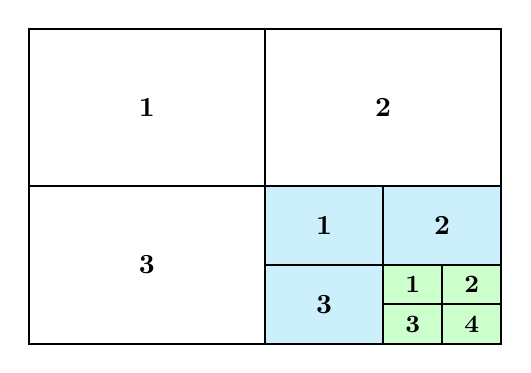
\begin{tikzpicture}
        
            % Duży prostokąt
            \draw[thick] (0, 0) rectangle (6, 4);
        
            % Linie podziału dużego prostokąta (ćwiartki)
            \draw[thick] (3, 0) -- (3, 4);
            \draw[thick] (0, 2) -- (6, 2);
        
            % Numery ćwiartek w dużym prostokącie
            \node at (1.5, 3) {\textbf{1}};
            \node at (4.5, 3) {\textbf{2}};
            \node at (1.5, 1) {\textbf{3}};
            \node at (4.5, 1) {\textbf{4}};
        
            % Mały prostokąt (ćwiartka 4)
            \draw[thick, fill=cyan!20] (3, 0) rectangle (6, 2);
        
            % Linie podziału małego prostokąta (ćwiartki ćwiartki)
            \draw[thick] (4.5, 0) -- (4.5, 2);
            \draw[thick] (3, 1) -- (6, 1);
        
            % Numery ćwiartek w małym prostokącie
            \node at (3.75, 1.5) {\textbf{1}};
            \node at (5.25, 1.5) {\textbf{2}};
            \node at (3.75, 0.5) {\textbf{3}};
            \node at (5.25, 0.5) {\textbf{4}};
        
            % Podział ćwiartki 4 w małym prostokącie (zielony)
            \draw[thick, fill=green!20] (4.5, 0) rectangle (6, 1);
            \draw[thick] (5.25, 0) -- (5.25, 1);
            \draw[thick] (4.5, 0.5) -- (6, 0.5);
        
            % Numery ćwiartek w zielonym obszarze
            \node at (4.875, 0.75) {\small \textbf{1}};
            \node at (5.625, 0.75) {\small \textbf{2}};
            \node at (4.875, 0.25) {\small \textbf{3}};
            \node at (5.625, 0.25) {\small \textbf{4}};
        
            \end{tikzpicture}
        \end{center}
    \end{column}

\end{columns}
    
\end{frame}

\end{section}

\begin{section}{\texttt{Kd-drzewa}}

\begin{frame}{Ogólna idea \texttt{kd-drzewo}}
    \textbf{Dlaczego kd-drzewo?}\\
    \vspace{0.4em}
    \begin{itemize}
        \item \texttt{kd-drzewo} (k-d Tree) to struktura do przechowywania punktów 
              w przestrzeniach wielowymiarowych (u nas 2D).
        \item Zamiast traktować wszystkie wymiary naraz, dzielimy przestrzeń 
              po jednej osi na danym poziomie drzewa (np. raz po \(x\), raz po \(y\)).
        \item Taki rekurencyjny podział sprawia, że do wielu zapytań przestrzennych
              (np. \textit{czy punkt A leży w danym obszarze?})
              nie musimy przeglądać wszystkich danych, a tylko część drzewa.
        \item Dzięki temu kd-drzewo często \textit{znacznie przyspiesza wyszukiwanie} 
              w porównaniu z metodami naiwnymi, 
              zwłaszcza przy dużych zbiorach punktów.
    \end{itemize}
\end{frame}

\begin{frame}
        \frametitle{\texttt{kd-drzewo} -- teoretyczna złożoność}
            
        \begin{itemize}
            \item \textbf{Budowa struktury:}  
            \(\Theta(n \log n)\), gdzie \(n\) to liczba punktów w zbiorze, przy założeniu równomiernego rozkładu punktów.
        \pause
        \vspace{0.5cm}
            \item \textbf{Wyszukiwanie punktów w zadanym obszarze:}  
        \(\Theta(\sqrt{n} + k)\), gdzie:
        \begin{itemize}
            \item \(\sqrt{n}\) to liczba węzłów jakie odwiedzi algorytm przy założeniu równomiernego rozkładu,
            \item \(k\) to liczba punktów wewnątrz zadanego obszaru.  
        \end{itemize}
        Dzięki rekurencyjnemu podziałowi przestrzeni wyszukiwanie jest ograniczone tylko do podobszarów przecinających zadany obszar, co znacząco poprawia efektywność.
        \end{itemize}
    
    \end{frame}

\begin{frame}{Budowa \texttt{kd-drzewa} (opis kroków)}

\begin{mdframed}
\textbf{Krok 1: Wybór osi podziału}\\[3pt]
Na podstawie aktualnego poziomu drzewa (\textit{głębokości}) decydujemy, czy dzielimy względem osi \(x\), czy \(y\).
- Jeśli głębokość jest parzysta (0, 2, 4, ...), to dzielimy względem \(x\).
- Jeśli nieparzysta (1, 3, 5, ...), to dzielimy względem \(y\).
\end{mdframed}

\begin{mdframed}
\textbf{Krok 2: Wybór punktu podziału (mediana)}\\[3pt]
Zbieramy listę punktów i sortujemy je według współrzędnej, która odpowiada wybranej osi.
Następnie \textit{mediana} (środkowy punkt w posortowanej liście) zostaje węzłem głównym
naszego poddrzewa. \\
\textit{Dzięki temu drzewo jest w miarę zbalansowane, bo po obu stronach mediany jest podobna liczba punktów.}
\end{mdframed}

    
\end{frame}

\begin{frame}{Budowa \texttt{kd-drzewa} (opis kroków) -- c.d.}
\begin{mdframed}
\textbf{Krok 3: Podział zbioru punktów} \\[3pt]
Wszystkie punkty, które w wybranym wymiarze są „mniejsze” od mediany,
przydzielamy do lewego poddrzewa, a punkty „większe” – do prawego poddrzewa.  
\textit{Jeżeli os to \(x\), to dzielimy: \((x \leq x_{\text{mediany}})\) \(\to\) lewa strona, a \((x > x_{\text{mediany}})\) \(\to\) prawa strona.}
\end{mdframed}

\begin{mdframed}
\textbf{Krok 4: Rekurencja} \\[3pt]
Powyższe czynności powtarzamy dla „lewego” i „prawego” zbioru – znów sprawdzając kolejną
oś (naprzemiennie). Proces kończy się, kiedy w danym węźle
pozostanie już pojedynczy punkt lub zbiór będzie pusty.
\end{mdframed}

\end{frame}

\begin{frame}{Wizualizacja budowy \texttt{kd-drzewa}}
    \centering
    % Adjust the width as needed (e.g., 0.8\linewidth)
    \animategraphics[
        autoplay,    % Start playing automatically
        loop,        % Loop the animation continuously
        controls,
        width=0.71\linewidth
    ]{4}{gif_kd/frame_}{1}{63}
    % % Parameters:
    % % 10       - Frame rate (frames per second)
    % % frame_   - Prefix of the frame image files
    % % 0000     - Starting frame number
    % % 0020     - Ending frame number (adjust based on your frames)
\end{frame}

\begin{frame}{Wyszukiwanie punktów w obszarze \([x_1, x_2] \times [y_1, y_2]\)}

\begin{mdframed}
\textbf{Krok 1: Sprawdzenie punktu w aktualnym węźle}\\[3pt]
Rozpoczynamy od korzenia drzewa i sprawdzamy, czy punkt w tym węźle
(zapamiętana mediana) mieści się w obszarze \([x_1, x_2] \times [y_1, y_2]\).
Jeżeli tak – dodajemy go do wyniku.
\end{mdframed}

\begin{mdframed}
\textbf{Krok 2: Analiza podziału drzewa} \\[3pt]
Patrzymy, w którą stronę naszego obszaru \textit{mogą} spadać interesujące nas punkty.
- Jeśli dzielimy względem \(x\) i nasza lewa granica \((x_1)\) jest mniejsza bądź równa od współrzędnej \(x\) bieżącego punktu,
  to \textbf{wiemy}, że w lewym poddrzewie mogą być punkty w zakresie.  
- Z kolei, jeśli prawa granica \((x_2)\) jest większa bądź równa od tej współrzędnej,
  to idziemy też w prawo.
- Analogicznie postępujemy, gdy podział jest względem \(y\).
\end{mdframed}

\end{frame}
\begin{frame}{Wyszukiwanie punktów w obszarze \([x_1, x_2] \times [y_1, y_2]\) -- c.d.}
\begin{mdframed}
\textbf{Krok 3: Rekurencja} \\[3pt]
Przechodzimy do węzłów lewego i/lub prawego, powtarzając ten sam schemat:
- Czy punkt węzła mieści się w zakresie?
- Czy warto iść dalej w lewo/prawo, biorąc pod uwagę porównanie
  współrzędnej węzła z \([x_1, x_2]\) albo \([y_1, y_2]\)?

\textit{Dzięki temu „omijamy” poddrzewa, które na pewno nie mają punktów w naszym obszarze.}
\end{mdframed}

\begin{mdframed}
\textbf{Krok 4: Zakończenie wyszukiwania}\\[3pt]
Kiedy dotrzemy do pustych węzłów lub przejdziemy przez całe drzewo w miejsca
potencjalnie zawierające punkty w zakresie, kończymy rekurencję.  
Wszystkie punktu zebrane po drodze \emph{muszą} być tymi, które leżą
w zadanym prostokącie \([x_1, x_2] \times [y_1, y_2]\).
\end{mdframed}

\end{frame}
\begin{frame}{Wizualizacja zapytania dla \texttt{kd-drzewa}}
\begin{center}
    \includegraphics[width=0.8\linewidth]{points.png}
\end{center}
\end{frame}
\begin{frame}{Wizualizacja zapytania dla \texttt{kd-drzewa}}
        \centering
    % Adjust the width as needed (e.g., 0.8\linewidth)
    \animategraphics[
        autoplay,    % Start playing automatically
        loop,        % Loop the animation continuously
        controls,
        width=0.84\linewidth
    ]{2}{gif_kd_zapytanie/frame_}{1}{14}
    % Parameters:
    % 10       - Frame rate (frames per second)
    % frame_   - Prefix of the frame image files
    % 0000     - Starting frame number
    % 0020     - Ending frame number (adjust based on your frames)
\end{frame}

\begin{frame}[fragile]{Budowa kd-drzewa w Pythonie i złożoność}
\vspace{0.3em}
\begin{itemize}
    \item \textbf{Dlaczego to może być \(O(n \log^2 n)\)?} 
    \begin{itemize}
      \item Na każdym poziomie drzewa sortujemy listę punktów (\(O(n \log n)\)), 
            a poziomów jest \(\log n\) w przypadku dość równomiernego podziału.
      \item Sumarycznie: \(O(n \log n)\) \(\times\) \(\log n = O(n \log^2 n)\).
    \end{itemize}
    
    \item \textbf{Czy da się osiągnąć \(O(n \log n)\)?} 
    \begin{itemize}
      \item Tak, np. używając szybkich algorytmów wyszukiwania mediany (Quickselect, Introselect) zamiast pełnego sortowania na każdym poziomie.
      \item Jednak w praktyce implementacja Quickselect/Introselect bywa bardziej skomplikowana i w gorszym przypadku może się źle skalować (np. Quickselect ma pesymistycznie \(O(n^2)\)). 
      \item Często prostota kodu (sortowanie) bywa ważniejsza niż teoretyczny zysk, zwłaszcza przy realnych danych.
    \end{itemize}
\end{itemize}

\end{frame}

\begin{frame}{Zastosowania \texttt{kd-drzewa}}
    \begin{itemize}
        \item \textbf{Wyszukiwanie najbliższych sąsiadów (ang. Nearest Neighbor Search):}
        \begin{itemize}
            \item \(\,k\)-NN w uczeniu maszynowym (np. klasyfikacja, regresja).
            \item Znajdowanie najbardziej podobnych obiektów w dużych zbiorach danych.
        \end{itemize}
        \vspace{-0.1em}
        
        \item \textbf{Zapytania przestrzenne:}
        \begin{itemize}
            \item Wyszukiwanie punktów w zadanym obszarze (prostokącie, kuli itp.).
            \item Optymalizacja zapytań GIS, np. w bazach danych geograficznych.
        \end{itemize}
        \vspace{-0.1em}
        
        \item \textbf{Klasteryzacja i analiza danych wielowymiarowych:}
        \begin{itemize}
            \item Skupiska punktów w 2D lub wyższych wymiarach.
            \item Przyspieszanie algorytmów typu DBSCAN, Mean Shift itp.
        \end{itemize}
        \vspace{-0.1em}
        
        \item \textbf{Wizualizacja i grafika komputerowa:}
        \begin{itemize}
            \item Struktura przyspieszająca techniki renderowania (np. \emph{ray tracing}).
            \item Wspomaganie detekcji kolizji w symulacjach i grach 2D/3D.
        \end{itemize}
        \vspace{-0.1em}
        
        \item \textbf{Systemy rzeczywiste:}
        \begin{itemize}
            \item Aplikacje robotyczne (wyznaczanie najbliższych przeszkód).
            \item Motory rekomendujące (wielowymiarowe porównywanie cech produktów).
        \end{itemize}
    \end{itemize}
\end{frame}
\begin{frame}{Generalizacja do k-wymiarów}
\begin{center}
    \includegraphics[width=0.6\linewidth]{3dtree.png}
\end{center}
\end{frame}
\end{section}
\begin{section}{Porównanie struktur}

\begin{frame}{\texttt{kd-drzewo} vs \texttt{QuadTree} -- Różnice w strukturze}
    \begin{itemize}
        \item \textbf{Podział przestrzeni:}
            \begin{itemize}
                \item \texttt{kd-drzewo}: na każdym poziomie dzielimy przestrzeń względem jednej osi (x lub y), naprzemiennie.
                \item \texttt{QuadTree}: na każdym poziomie dzielimy przestrzeń na cztery równe ćwiartki (osie x i y jednocześnie).
            \end{itemize}
            \vspace{0.4em}
            
        \item \textbf{Układ węzłów drzewa:}
            \begin{itemize}
                \item \texttt{kd-drzewo}: węzeł przechowuje pojedynczy punkt (mediana dla danej osi). Dzieli się na \emph{lewe} i \emph{prawe} poddrzewo.
                \item \texttt{QuadTree}: węzeł może przechowywać wiele punktów (do pewnego limitu), potem następuje podział zwykle na cztery poddrzewa (\emph{NW}, \emph{NE}, \emph{SW}, \emph{SE}).
            \end{itemize}
            \vspace{0.4em}
            
        \item \textbf{Wielowymiarowość:}
            \begin{itemize}
                \item \texttt{kd-drzewo}: naturalnie rozszerza się na \(k\) wymiarów (stąd nazwa).
                \item \texttt{QuadTree}: typowo używane w 2D, choć istnieją analogie (tzw. \texttt{OctTree} w 3D).
            \end{itemize}
    \end{itemize}
\end{frame}

\begin{frame}{\texttt{kd-drzewo} vs \texttt{QuadTree} -- Złożoność i zastosowania}
    \begin{block}{Złożoność i efektywność}
    \begin{itemize}
        \item \textbf{Budowa:}
            \begin{itemize}
                \item \texttt{kd-drzewo}: często \(O(n \log n)\) (przy równomiernym rozkładzie i efektywnym wybieraniu median).  
                \item \texttt{QuadTree}: \(O(n \log n)\) przy równomiernym rozkładzie, choć implementacja oparta jest na iteracyjnym podziale przestrzeni, a nie na wyszukiwaniu median.
            \end{itemize}
        \item \textbf{Wyszukiwanie:}
            \begin{itemize}
                \item \texttt{kd-drzewo}: Średnio \(O(\sqrt{n} + k)\) w 2D, gdzie \(k\) to liczba punktów w obszarze.
                \item \texttt{QuadTree}: Także średnio \(O(\log n + k)\), przy założeniu równomiernego rozkładu (a w praktyce bywa różnie).
            \end{itemize}
    \end{itemize}
    \end{block}
\end{frame}

\begin{frame}{Kiedy wybrać \texttt{kd-drzewo} a kiedy \texttt{QuadTree}?}
    \textbf{Podsumowanie kryteriów wyboru:}
    \begin{itemize}
        \item \(\,k\geq 3\):  
              \(\rightarrow\) \texttt{kd-drzewo} naturalnie się rozszerza na \(k\) wymiarów, \texttt{QuadTree} (2D) nie.  
              (\texttt{OctTree} jest 3D analogią Quadtree, ale bywa bardziej złożony w implementacji.)
        \item \(\,\) \textbf{Wyszukiwanie w obszarze vs. Wyszukiwanie najbliższych sąsiadów:}
            \begin{itemize}
                \item \texttt{kd-drzewo} jest często lepsze do najbliższych sąsiadów, szczególnie w 2D/3D.
                \item \texttt{QuadTree} wystarczająco dobrze radzi sobie z przeszukiwaniem obszarów, szczególnie przy równomiernym rozkładzie w 2D.
            \end{itemize}
        \item \(\,\) \textbf{Implementacja i prostota}:
            \begin{itemize}
                \item \texttt{QuadTree} – dość prosty kod (rekurencyjny podział na 4 ćwiartki).
                \item \texttt{kd-drzewo} – wymaga wyznaczania mediany (lub sortowania) przy budowie, ale jest dość uniwersalny w wymiarach \(>2\).
            \end{itemize}
    \end{itemize}
\end{frame}

% Zostawić czy wywalić taki zbiorczy slajd na koniec??? Bo nawet ładny
\begin{frame}{Zastosowania}
    \begin{block}{Typowe zastosowania}
    \begin{itemize}
        \item \texttt{kd-drzewo}:
            \begin{itemize}
                \item Wyszukiwanie najbliższych sąsiadów (\emph{ang. Nearest Neighbor Search}).
                \item Klasteryzacja w przestrzeniach wielowymiarowych.
                \item Zapytania typu przeszukiwanie obszaru (dla 2D, 3D i więcej wymiarów).
            \end{itemize}
            
        \item \texttt{QuadTree}:
            \begin{itemize}
                \item Zadania stricte 2D: grafika komputerowa, operacje na obrazach, GIS.
                \item Renderowanie terenu, kolizje w grach 2D.
                \item Kompresja i segmentacja obrazów (\emph{przetwarzanie obrazów}).
            \end{itemize}
    \end{itemize}
    \end{block}
\end{frame}
    \begin{frame}{}
      \centering \Large
      \emph{Zobaczmy jak to wygląda w kodzie}
    \end{frame}
\end{section}

\begin{frame}{}
  \centering \Huge
  \emph{Koniec. Dziękujemy za uwagę!}
\end{frame}

\end{document}
